% !TeX root = ../../main.tex
\documentclass[../AAE590LGM_HW3.tex]{subfiles}
\begin{document}

\subsection{3.a) \textbf{Group Operations:}}
\underline{Question}: \\
Implement $\SEt{2}$ compose and inverse \\
\underline{Solution}: \\
Code snippet 3 shows the implementation of \texttt{se22\_compose(X1, X2)} and \texttt{se22\_inverse(X)}
Code snippet 4 shows its unit test and Fig \ref{fig:set2utestpass} shows its passing.

\subsection{3.b) \textbf{Lie Algebra $\set{2}$:}}
\underline{Question}: \\
Implement \texttt{se22\_wedge(xi)} and \texttt{se22\_vee(Xi)} \\
\underline{Solution}: \\
Code snippet 3 shows the implementation of \texttt{se22\_wedge(xi)} and \texttt{se22\_vee(Xi)}
Code snippet 4 shows its unit test and Fig \ref{fig:set2utestpass} shows its passing.

\subsection{3.c) \textbf{Exponential and Logarithm Maps:}}
\underline{Question}: \\
Implement \texttt{se22\_exp(xi)} and \texttt{se22\_log(X)}. Verify round-trip: $\Exp\!\bigl((\Log(X))^\wedge\bigr) = X$ for at least 3 random $X \in \SEt(2)$ (i.e., \texttt{se22\_exp(se22\_log(X))} recovers $X$ to machine precision). \\
\underline{Solution}: \\
Code snippet 3 shows the implementation of \texttt{se22\_exp(xi)} and \texttt{se22\_log(X)}. \\
Code snippet 4 shows its unit test and Fig \ref{fig:set2utestpass} shows its passing.

\subsection{3.d) \textbf{Adjoint $\Ad_X$ and Small Adjoint $\ad_\xi$:}}
\underline{Question}: \\
Implement \texttt{se22\_Ad(X)} and \texttt{se22\_ad(xi)}. Verify numerically (for at least 3 random inputs each):
\begin{itemize}
    \item $\Ad_{X_1 X_2} = \Ad_{X_1} \Ad_{X_2}$
    \item $[\xi_1, \xi_2] = \ad_{\xi_1} \xi_2$
\end{itemize}
\underline{Solution}: \\
Code snippet 3 shows the implementation of the functions \texttt{se22\_Ad(X)} and \texttt{se22\_ad(xi)}.
Code snippet 4 shows the implementation of the unit test verifying $\Ad_{X_1 X_2} = \Ad_{X_1} \Ad_{X_2}$ for random $X_1, X_2 \in \SEt{2}$ for random $X \in \SEt{2}$ named \texttt{test\_se22\_Ad\_composition} and Fig \ref{fig:set2utestpass} shows the test passing.
Code snippet 4 shows the implementation of the unit test verifying $[\xi_1, \xi_2] = \ad_{\xi_1} \xi_2$ for random $\xi_1, \xi_2 \in \set{2}$ named \texttt{test\_se22\_ad} and Fig \ref{fig:set2utestpass} shows the test passing.

\subsection{Implementation and Unit Tests}
\lstinputlisting[language=Python,caption={$\SEt{2}$ and $\set{2}$ Function Implementations}, inputpath=../../../Code/SE22]{SE22_maps.py}

\lstinputlisting[language=Python,caption={Unit Tests for $\SEt{2}$ Using Pytest}, inputpath=../../../Tests/SE22]{test_SE22.py}

\begin{figure}[H]
    \caption{Pytest unit test output showing tests passing}
    \centering
    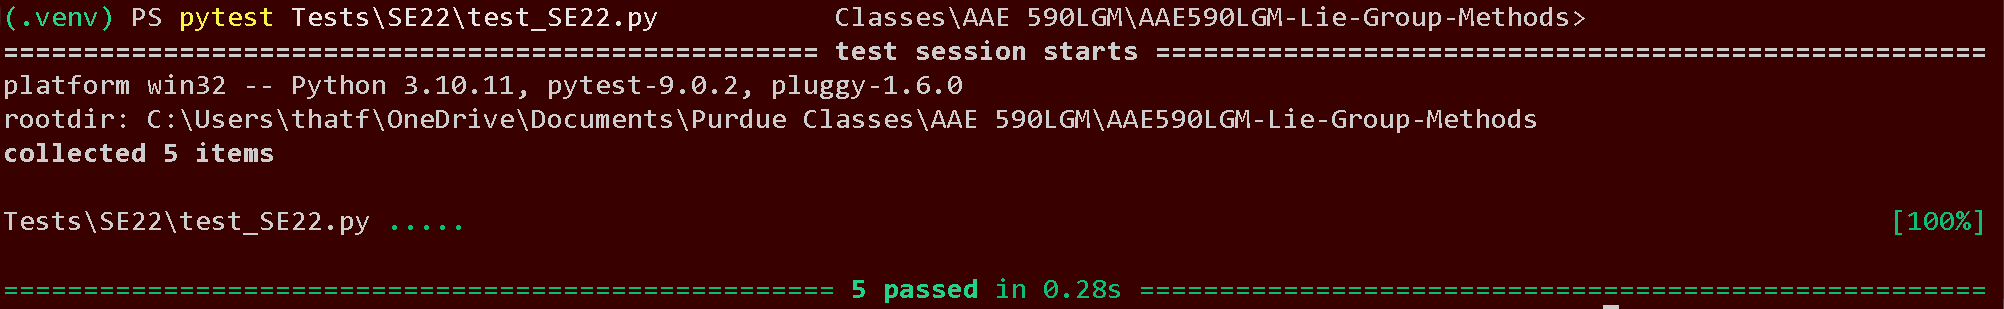
\includegraphics[width=1\linewidth]{AAE590LGM_HW3_Q3_SE22_utests.png}
    \label{fig:set2utestpass}
\end{figure}


\end{document}